\chapter{Fotochemie}\label{ch:b3:photochemistry}

Zien begint wanneer één foton één molecuul ombuigt. In de staafjes van het
oog zit retinal in zijn eiwit in de 11-cisvorm; een foton groen licht zet
het om in de all-transvorm, en de isomerisatie is in essentie voltooid
binnen \qty{200}{fs}, sneller dan bijna elk ander chemisch proces. De rest
van het zien, een enorme biochemische versterking, volgt uit dat ene
omgebogen molecuul. Dezelfde regels (één foton slaat één molecuul aan, dat
daarna kiest tussen meerdere lotsbestemmingen) gelden voor zonnecrèmes,
de synthese van gespannen ringen, fotodynamische therapie, de smog boven
steden en de \omterm{def:b3:photochemistry:chapman}{ozonlaag} die het aardoppervlak beschermt tegen ultraviolet
licht.

\begin{recall}
\Cref{ch:b3:electronic-spectroscopy} beschreef de aangeslagen toestanden
van moleculen, het \omterm{def:b3:electronic-spectroscopy:jablonski}{jablonskidiagram}, \omterm{def:b3:electronic-spectroscopy:radiationless}{intersystem crossing}, \omterm{def:b3:electronic-spectroscopy:luminescence}{fluorescentie}
en \omterm{def:b3:electronic-spectroscopy:luminescence}{fosforescentie}, uitdoving en de \omterm{def:b3:electronic-spectroscopy:quantum-yield}{kwantumopbrengst} van een fotofysisch
proces. Het deel van jaar~1 definieerde radicalen, homolyse en
$Z$/$E$-isomeren; het deel van jaar~2
gecoördineerde reacties, grensorbitalen en katalytische cycli.
\Cref{ch:b3:complex-kinetics} behandelde \omterm{def:b3:complex-kinetics:chain}{kettingreacties} en stationaire
toestanden.
\end{recall}

\section{Licht als reagens}

Twee oude principes openen het onderwerp: alleen licht dat geabsorbeerd
wordt, kan een chemische verandering veroorzaken (Grotthuss en Draper), en
elk geabsorbeerd foton slaat één molecuul aan (Stark en Einstein).

\begin{definition}[Fotonenflux, chemische actinometer]\label{def:b3:photochemistry:photon-flux}
De \emph{fotonenflux}\index{fotonenflux} van een lichtbron is het aantal
fotonen dat ze per tijdseenheid levert, vaak geteld in mol fotonen
(einstein) per seconde. Een
\emph{chemische actinometer}\index{chemische actinometer} is een
fotochemische reactie met een nauwkeurig bekende \omterm{def:b3:electronic-spectroscopy:quantum-yield}{kwantumopbrengst}, die
gebruikt wordt om een fotonenflux te meten.
\end{definition}

\begin{proposition}[Wet van Stark-Einstein]\label{prop:b3:photochemistry:stark-einstein}
Bij gewone lichtintensiteiten slaat elk geabsorbeerd foton precies één
molecuul aan; de primaire \omterm{def:b3:electronic-spectroscopy:quantum-yield}{kwantumopbrengsten} van alle processen die
vanuit de aangeslagen toestand vertrekken, tellen op tot 1.
\end{proposition}

\begin{proof}[Gedeeltelijk bewijs]
Dat één foton tegelijk door één molecuul geabsorbeerd wordt, wordt
aangenomen (tweefotonabsorptie vereist de intensiteiten van gepulste
lasers). Het aangeslagen molecuul verdwijnt daarna via concurrerende
processen van de eerste orde met snelheidsconstanten $k_i$
(\cref{ch:b3:electronic-spectroscopy}): de fractie die weg $i$ volgt, is $\Phi_i =
k_i/\sum_jk_j$, en $\sum_i\Phi_i = 1$.
\end{proof}

De \omterm{def:b3:electronic-spectroscopy:quantum-yield}{kwantumopbrengst} van een reactie, het aantal omgezette moleculen per
geabsorbeerd foton, hoeft deze limiet niet te respecteren: een primaire
fotochemische stap kan een keten starten. Een mengsel van \ce{H2} en
\ce{Cl2} dat aan licht blootgesteld wordt, reageert met
\omterm{def:b3:electronic-spectroscopy:quantum-yield}{kwantumopbrengsten} van $10^4$ en meer, waarbij elk gefotolyseerd
\ce{Cl2} een keten start zoals die van de reactie van waterstof met broom
in \cref{ch:b3:complex-kinetics}; een \omterm{def:b3:electronic-spectroscopy:quantum-yield}{kwantumopbrengst} groter dan 1 is
het kenmerk van een keten.

\begin{proposition}[Snelheid van een fotochemische reactie]\label{prop:b3:photochemistry:rate}
Een oplossing met absorbantie $A$ bij de bestralingsgolflengte, die een
\omterm{def:b3:photochemistry:photon-flux}{fotonenflux} $I_0$ (einstein per seconde) ontvangt, absorbeert $I_{\mathrm{abs}} = I_0(1 - 10^{-A})$; als de
beginstof alles absorbeert, zet de reactie $v = \Phi I_{\mathrm{abs}}$ mol per seconde om.
\end{proposition}

\begin{proof}
Volgens de wet van Lambert-Beer is de doorgelaten flux $I_010^{-A}$, zodat
de geabsorbeerde flux
$I_0(1 - 10^{-A})$ is; volgens de definitie van de \omterm{def:b3:electronic-spectroscopy:quantum-yield}{kwantumopbrengst}
reageren er $\Phi$ moleculen per geabsorbeerd foton.
\end{proof}

\begin{method}[De snelheid van een fotoreactie uit de lamp]\label{met:b3:photochemistry:photochemical-rate}
\begin{enumerate}
  \item Fotonenergie $E = hc/\lambda$; \omterm{def:b3:photochemistry:photon-flux}{fotonenflux} $I_0 = P/E$ voor een
        vermogen $P$ dat het monster bereikt, of gemeten met een
        actinometer; deel door $N_A$ voor einstein per seconde.
  \item Geabsorbeerde fractie $1 - 10^{-A}$, met $A$ bij de
        bestralingsgolflengte (ze verandert naarmate de beginstof
        verbruikt wordt).
  \item Snelheid $\Phi I_{\mathrm{abs}}$ in mol/s, gedeeld door het volume
        voor een concentratiesnelheid.
\end{enumerate}
\end{method}

\begin{method}[Ferrioxalaatactinometrie]\label{met:b3:photochemistry:actinometry}
\begin{enumerate}
  \item Bestraal, in dezelfde cel en dezelfde geometrie als het experiment,
        een aangezuurde oplossing van kaliumtris(oxalato)ferraat(III),
        geconcentreerd genoeg om praktisch al het licht onder ongeveer
        \qty{450}{nm} te absorberen.
  \item Licht reduceert Fe(III) tot Fe(II) met een gekalibreerde
        \omterm{def:b3:electronic-spectroscopy:quantum-yield}{kwantumopbrengst}; voeg na een gemeten tijd 1,10-fenantroline en een
        buffer toe, en meet de absorbantie van het rode complex $\ce{[Fe(phen)3]^{2+}}$.
  \item Het aantal mol Fe(II) gedeeld door (\omterm{def:b3:electronic-spectroscopy:quantum-yield}{kwantumopbrengst} $\times$ tijd)
        geeft de \omterm{def:b3:photochemistry:photon-flux}{fotonenflux}.
\end{enumerate}
\end{method}

\section{Fotochemische reacties}

\begin{definition}[Foto-isomerisatie, fotostationaire toestand]\label{def:b3:photochemistry:photoisomerisation}
Een \emph{foto-isomerisatie}\index{foto-isomerisatie} is een door licht
veroorzaakte omzetting van een isomeer in een ander, typisch $E \to Z$ rond een dubbele binding. Onder
continue bestraling bereiken twee isomeren die beide absorberen een
\emph{fotostationaire toestand}\index{fotostationaire toestand}, een
stabiele samenstelling die door het licht bepaald wordt, niet door de
thermodynamica.
\end{definition}

Het verdraaien van een dubbele binding verklaart waarom licht alkenen
isomeriseert. In de grondtoestand stijgt de energie naarmate de twee
uiteinden verdraaien, tot een maximum bij $90^\circ$, waar de $\pi$-binding
verbroken is. In de aangeslagen toestand $\pi\pi^*$ is de volgorde
omgekeerd: de verdraaide geometrie is de stabielste. Een aangeslagen
molecuul draait naar
$90^\circ$, waar de twee oppervlakken samenkomen, gaat daar terug naar de
grondtoestand, en valt naar een van beide kanten: naar het isomeer
waarvan het vertrok of naar het andere.

\begin{omfigure}
\begin{tikzpicture}[font=\small, >=Stealth, x=0.032cm, y=1.1cm]
  \draw[->] (0,0) -- (195,0);
  \node[anchor=north] at (135,-0.45) {torsiehoek};
  \draw[->] (0,0) -- (0,5.2) node[anchor=south] {energie};
  \foreach \t/\l in {0/{0^\circ}, 90/{90^\circ}, 180/{180^\circ}}{
    \draw (\t,0) -- (\t,-0.08) node[anchor=north] {$\l$};}
  \draw[thick, black, domain=0:180, samples=90] plot (\x,{2.6*sin(\x)^2 + 0.15*(1-cos(\x))/2});
  \draw[thick, omThm, domain=0:180, samples=90] plot (\x,{4.5 - 1.6*sin(\x)^2 + 0.1*(1-cos(\x))/2});
  \node[anchor=east] at (0,0.15) {$E$};
  \node[anchor=west] at (182,0.2) {$Z$};
  \node[omThm, anchor=south west] at (5,4.55) {$\mathrm S_1$ ($\pi\pi^*$)};
  \node[anchor=north west] at (52,1.2) {$\mathrm S_0$};
  \draw[->, omDef, thick] (12,0.12) -- (12,4.4) node[midway, left] {$h\nu$};
  \draw[->, omDef, thick, decorate, decoration={snake, amplitude=0.6mm, segment length=3mm}] (16,4.4) -- (80,3.05);
  \draw[->, omDef, thick] (90,2.85) -- (90,2.75);
  \draw[->, black!60, thick, domain=96:168, samples=40] plot (\x,{2.6*sin(\x)^2 + 0.15*(1-cos(\x))/2 + 0.28});
  \draw[->, black!60, thick, domain=84:12, samples=40] plot (\x,{2.6*sin(\x)^2 + 0.15*(1-cos(\x))/2 + 0.28});
  \node[font=\scriptsize, anchor=south, align=center] at (90,3.45) {trechter};
\end{tikzpicture}

{\small Grondtoestand ($\mathrm S_0$) en eerste aangeslagen toestand
($\mathrm S_1$) van een alkeen als functie van de verdraaiing van zijn
dubbele binding (schematisch). Excitatie van het $E$-isomeer (verticale
pijl) wordt gevolgd door verdraaiing op $\mathrm S_1$ tot de loodrechte
geometrie, waar de twee oppervlakken elkaar bijna raken; het molecuul
keert daar terug naar $\mathrm S_0$ en relaxeert naar $E$ of naar
$Z$.}
\end{omfigure}

\begin{proposition}[Fotostationaire samenstelling]\label{prop:b3:photochemistry:pss}
Onder monochromatische bestraling van een optisch dunne oplossing
bereiken twee isomeren $E$
en $Z$ met absorptiecoëfficiënten $\varepsilon_E$, $\varepsilon_Z$ en \omterm{def:b3:electronic-spectroscopy:quantum-yield}{kwantumopbrengsten} $\Phi_{E\to Z}$,
$\Phi_{Z\to E}$ de fotostationaire verhouding
\[
  \frac{[Z]}{[E]} = \frac{\varepsilon_E\Phi_{E\to Z}}{\varepsilon_Z\Phi_{Z\to E}} .
\]
\end{proposition}

\begin{proof}
In een optisch dun monster absorbeert elk isomeer een flux die evenredig
is met $\varepsilon[\cdot]$, zodat
$\dd[Z]/\dd t = c(\varepsilon_E\Phi_{E\to Z}[E] - \varepsilon_Z\Phi_{Z\to E}[Z])$ met een constante $c$ die het licht vastlegt;
de stationaire toestand maakt de uitdrukking tussen haken nul. (Het
resultaat geldt ook voor dikke monsters, omdat de twee isomeren het
geabsorbeerde licht dan in dezelfde verhouding delen.)
\end{proof}

\begin{omfigure}
\begin{tikzpicture}
\begin{axis}[width=0.7\linewidth, height=5.0cm, xmin=0, xmax=120, ymin=0, ymax=1,
  axis lines=left, xlabel={bestralingstijd / s}, ylabel={fractie $Z$},
  tick label style={font=\small}, label style={font=\small}]
\addplot[omDef, very thick] table[x=t, y=Z] {figdata/out/bachelor-3-photostationary.dat};
\draw[black!35, densely dotted] (axis cs:0,0.801) -- (axis cs:60,0.801);
\draw[black!35, densely dotted] (axis cs:60,0.161) -- (axis cs:120,0.161);
\draw[black!35] (axis cs:60,0) -- (axis cs:60,1);
\node[font=\scriptsize, anchor=north] at (axis cs:30,0.98) {\qty{365}{nm}};
\node[font=\scriptsize, anchor=north] at (axis cs:90,0.98) {\qty{440}{nm}};
\node[font=\scriptsize, anchor=south east] at (axis cs:58,0.81) {fst 0.80};
\node[font=\scriptsize, anchor=south east] at (axis cs:118,0.17) {fst 0.16};
\end{axis}
\end{tikzpicture}

{\small Een modelfotoschakelaar (een molecuul van het type azobenzeen),
bestraald bij \qty{365}{nm}, waar het $E$-isomeer veel sterker absorbeert,
en daarna bij \qty{440}{nm}, waar het $Z$-isomeer dat doet: de
samenstelling schakelt tussen twee \omterm{def:b3:photochemistry:photoisomerisation}{fotostationaire toestanden} (fst; model
voor de absorptiecoëfficiënten en \omterm{def:b3:electronic-spectroscopy:quantum-yield}{kwantumopbrengsten}).}
\end{omfigure}

De isomerisatie van 11-cis- naar all-transretinal in rodopsine is zo'n
reactie, die door het eiwit uitzonderlijk snel en selectief gemaakt
wordt. Synthetische fotoschakelaars op basis van azobenzeen of stilbeen
worden gebruikt om moleculaire machines, materialen en, gekoppeld aan
geneesmiddelen of ionkanalen, biologische activiteit met licht te sturen.

\begin{definition}[Fotolyse]\label{def:b3:photochemistry:photolysis}
\emph{Fotolyse}\index{fotolyse} is het verbreken van een binding door
licht. In de atmosfeer telt de snelheidsconstante van de eerste orde $j$
van de fotolyse van een deeltje, zijn
\emph{fotolysesnelheidsconstante}\index{fotolysesnelheidsconstante}, over
alle golflengten de \omterm{def:b3:photochemistry:photon-flux}{fotonenflux} van de zon op, maal de
absorptiedoorsnede, maal de \omterm{def:b3:electronic-spectroscopy:quantum-yield}{kwantumopbrengst}.
\end{definition}

Een foton verbreekt een binding alleen als zijn energie groter is dan de
dissociatie-energie:
$\lambda < hcN_A/D_0$. Voor \ce{O2} is $D_0 = 2\Delta_fH^\circ_0(\ce{O}) = \qty{493.6}{kJ/mol}$
volgens de thermochemische tabellen, en alleen licht korter dan
\qty{242}{nm} kan het splitsen.

Aangeslagen ketonen en alkenen vormen ook bindingen. Twee alkenen, waarvan
één aangeslagen, combineren tot een cyclobutaan: de
$[2+2]$-fotocycloadditie, verboden in de grondtoestand en toegestaan in de
aangeslagen toestand om orbitaalredenen die in \cref{ch:b3:pericyclic}
gegeven worden. Ze maakt vierringen, die gespannen en anders moeilijk
bereikbaar zijn, in één stap.

\begin{definition}[Norrishreacties]\label{def:b3:photochemistry:norrish}
Een \emph{norrishreactie van type I}\index{norrishreactie van type I} is
de splitsing, door een aangeslagen keton, van de binding tussen het
carbonylkoolstofatoom en een $\alpha$-koolstofatoom, in een acyl- en een
alkylradicaal. Een \emph{norrishreactie van type
II}\index{norrishreactie van type II} is de abstractie, door het
zuurstofatoom van een aangeslagen keton, van een waterstofatoom van het
$\gamma$-koolstofatoom, wat een 1,4-biradicaal geeft dat ofwel splitst in
een enol en een alkeen, ofwel sluit tot een cyclobutanol.
\end{definition}

\begin{omfigure}
\setchemfig{atom sep=1.9em}
\schemestart
\chemfig{H_3C-[:30]C(=[:90]O)-[:-30]CH_2-[:30]CH_2-[:-30]CH_2-[:30]CH_3}
\arrow{->[$h\nu$][via $\mathrm T_1$]}
\chemfig{H_3C-[:30]\chembelow{C}{\scriptstyle\bullet}(-[:90]OH)-[:-30]CH_2-[:30]CH_2-[:-30]\chemabove{C}{\scriptstyle\bullet}H-[:30]CH_3}
\schemestop

\medskip
\schemestart
\arrow{->[splitsing]}[,1.1]
\chemfig{H_3C-[:30]C(-[:90]OH)=[:-30]CH_2}
\+
\chemfig{H_2C=[:30]CH-[:-30]CH_3}
\schemestop
\hspace{2.5em}
\schemestart
\arrow{->[ring-][sluiting]}[,1.1]
\chemfig{*4(-(-[::-40]OH)(-[::40]CH_3)-(-CH_3)---)}
\schemestop
\par\medskip

{\small De \omterm{def:b3:photochemistry:norrish}{norrishreactie van type II} van hexaan-2-on. Het tripletketon
abstraheert een waterstofatoom van het $\gamma$-koolstofatoom via een
zesledige schikking; het 1,4-biradicaal splitst in het enol van aceton
(dat tautomeriseert tot aceton) en propeen, of sluit tot
1,2-dimethylcyclobutaan-1-ol.}
\end{omfigure}

De fotoreductie van benzofenon is de klassieke bimoleculaire variant: zijn
triplet abstraheert een waterstofatoom van een alcohol als oplosmiddel,
zoals propaan-2-ol, en twee van de gevormde
difenylhydroxymethylradicalen koppelen tot benzopinacol, dat uit de
oplossing kristalliseert.

\section{Fotosensibilisatie}

\begin{definition}[Fotosensibilisatie, singuletzuurstof]\label{def:b3:photochemistry:sensitisation}
Een \emph{fotosensibilisator}\index{fotosensibilisator} is een molecuul
dat licht absorbeert en de energie of een elektron overdraagt aan een
ander molecuul, dat zelf niet absorbeert: dit is
\emph{fotosensibilisatie}\index{fotosensibilisatie}. Bij
\emph{tripletenergieoverdracht}\index{tripletenergieoverdracht} geeft de
\omterm{def:b3:many-electron-atoms:singlet-triplet}{triplettoestand} van de sensibilisator, gevormd door \omterm{def:b3:electronic-spectroscopy:radiationless}{intersystem crossing},
bij contact zijn energie aan de acceptor, die in zijn \omterm{def:b3:many-electron-atoms:singlet-triplet}{triplettoestand}
achterblijft. \emph{Singuletzuurstof}\index{singuletzuurstof} is de
laagste aangeslagen toestand van \ce{O2},
${}^1\Delta_g$, die zo gevormd wordt uit zuurstof in de grondtoestand ${}^3\Sigma_g^-$.
\end{definition}

\begin{proposition}[Energievoorwaarde voor tripletoverdracht]\label{prop:b3:photochemistry:sensitisation-condition}
\omterm{def:b3:photochemistry:sensitisation}{Triplet-tripletenergieoverdracht} van een donor D naar een acceptor A
verloopt nagenoeg met de diffusielimiet wanneer $E_{\mathrm T}(\mathrm D)$
meer dan ongeveer \qty{10}{kJ/mol} groter is dan $E_{\mathrm T}(\mathrm A)$, en
daalt steil wanneer het verschil negatief wordt.
\end{proposition}

\begin{proof}[Gedeeltelijk bewijs]
De overdracht ${}^3\mathrm D + \mathrm A \to \mathrm D + {}^3\mathrm A$
behoudt de spin (twee tripletten geruild voor een singulet en een triplet)
en vereist orbitaalcontact (een uitwisselingsmechanisme, hier
aangenomen). Haar evenwichtsconstante is $\exp[(E_{\mathrm T}(\mathrm D) - E_{\mathrm T}(\mathrm A))/RT]$, ongeveer 60 voor een
overschot van \qty{10}{kJ/mol} bij \qty{298}{K}: de voorwaartse stap
gebeurt dan bij bijna elke ontmoeting. Wanneer het verschil negatief is,
is de voorwaartse snelheidsconstante de diffusielimiet maal het omgekeerde
van die factor (de bergop gerichte richting betaalt de boltzmannfactor);
de kwantitatieve kromme wordt aangenomen.
\end{proof}

Een goede sensibilisator absorbeert waar de acceptor dat niet doet, gaat
met een hoge opbrengst over naar zijn triplet, en heeft een lange
tripletlevensduur: benzofenon, met een tripletopbrengst van bijna 1, is de
standaard. \omterm{def:b3:photochemistry:sensitisation}{Singuletzuurstof} is een reactief elektrofiel: het addeert aan
diënen en aan elektronrijke alkenen. Bij fotodynamische therapie maakt
een sensibilisator die zich in een tumor ophoopt en via een optische vezel
belicht wordt, \omterm{def:b3:photochemistry:sensitisation}{singuletzuurstof} dat de omringende cellen vernietigt.

\begin{definition}[Fotoredoxkatalyse]\label{def:b3:photochemistry:photoredox}
\emph{Fotoredoxkatalyse}\index{fotoredoxkatalyse} gebruikt een
\omterm{def:b3:photochemistry:sensitisation}{fotosensibilisator} waarvan de aangeslagen toestand zowel een sterkere
oxidator als een sterkere reductor is dan de grondtoestand, om
afzonderlijke elektronen over te dragen naar of van substraten, wat onder
zichtbaar licht radicalen genereert; de sensibilisator wordt in een
katalytische cyclus geregenereerd.
\end{definition}

Het rutheniumcomplex $\ce{[Ru(bpy)3]^{2+}}$ is het prototype: zijn
aangeslagen toestand met ladingsoverdracht van metaal naar ligand,
bereikt met blauw licht en met een levensduur van ongeveer een
microseconde, kan een elektron opnemen van een amine of er een afstaan
aan een organisch halogenide. De gevormde radicalen nemen deel aan
reacties die bindingen vormen, onder veel mildere omstandigheden dan die
van de klassieke radicaalchemie.

\section{Fotochemie van de atmosfeer}

\begin{definition}[Mechanisme van Chapman, ozonlaag]\label{def:b3:photochemistry:chapman}
Het \emph{mechanisme van Chapman}\index{mechanisme van Chapman} is de reeks
van vier stappen
\[
  \ce{O2 ->[h\nu] 2 O}\ (j_1), \quad \mathrm{O + O_2 + M \to O_3 + M}\ (k_2), \quad
  \ce{O3 ->[h\nu] O2 + O}\ (j_3), \quad \ce{O + O3 -> 2 O2}\ (k_4).
\]
De \emph{ozonlaag}\index{ozonlaag} is het gebied van de stratosfeer,
ongeveer 15 tot \qty{35}{km} boven de grond, waar deze reacties de
grootste ozonconcentraties in stand houden.
\end{definition}

\begin{theorem}[Stationaire toestand van Chapman]\label{thm:b3:photochemistry:chapman}
In het \omterm{def:b3:photochemistry:chapman}{mechanisme van Chapman} bereiken O en \ce{O3} de stationaire toestand
\[
  \frac{[\ce{O}]}{[\ce{O3}]} = \frac{j_3}{k_2[\mathrm M][\ce{O2}]}, \qquad
  [\ce{O3}] = [\ce{O2}]\sqrt{\frac{j_1k_2[\mathrm M]}{j_3k_4}} .
\]
\end{theorem}

\begin{proof}
O en \ce{O3} gaan snel in elkaar over via de stappen 2 en 3 (seconden),
veel sneller dan ze gevormd of vernietigd worden: als men de snelle
uitwisseling in evenwicht stelt,
$k_2[\ce{O}][\ce{O2}][\mathrm M] = j_3[\ce{O3}]$, volgt de verhouding. Hun
som, de oneven zuurstof, wordt gevormd door stap 1 (twee O per \ce{O2})
en vernietigd door stap 4 (twee oneven zuurstofdeeltjes per gebeurtenis):
$2j_1[\ce{O2}] = 2k_4[\ce{O}][\ce{O3}]$. Invullen van $[\ce{O}]$ uit de verhouding geeft $[\ce{O3}]^2 = j_1k_2[\mathrm M][\ce{O2}]^2/(j_3k_4)$.
\end{proof}

Met de snelheidsconstanten uit de geëvalueerde databank en
fotolysesnelheden die typisch zijn voor \qty{30}{km} (gegevens van het
weekendprobleem) geeft het model van Chapman ongeveer
$\num{6e12}$ ozonmoleculen per \unit{cm^3}, zo'n vijftien delen per miljoen.
Geïntegreerd over de hoogte bevat de hele atmosfeer gemiddeld ongeveer 300
dobsoneenheden ozon: samengedrukt tot de druk aan het oppervlak, een laag
van \qty{3}{mm} dik. Het \omterm{def:b3:photochemistry:chapman}{mechanisme van Chapman} alleen voorspelt meer dan
waargenomen wordt: katalytische cycli breken ozon sneller af.

\begin{definition}[Ozonafbraak, reservoirverbinding]\label{def:b3:photochemistry:ozone-depletion}
\emph{Ozonafbraak}\index{ozonafbraak} is de afname van de stratosferische
ozonkolom door katalytische cycli van radicalen (Cl en ClO,
NO en \ce{NO2}, OH en \ce{HO2}). Een
\emph{reservoirverbinding}\index{reservoirverbinding}
is een stabiel molecuul (HCl, \ce{ClONO2}) dat een katalytisch radicaal in
een inactieve vorm vasthoudt, waaruit het later weer vrijgemaakt kan
worden.
\end{definition}

\begin{omfigure}
\begin{tikzpicture}[font=\small, >=Stealth]
  \node (cl) at (0,0) {Cl};
  \node (clo) at (3.2,0) {ClO};
  \draw[->, thick, omThm] (cl) to[bend left=40] node[midway, above] {$+\,\ce{O3}$, $-\,\ce{O2}$} (clo);
  \draw[->, thick, omThm] (clo) to[bend left=40] node[midway, below] {$+\,\ce{O}$, $-\,\ce{O2}$} (cl);
  \node[font=\scriptsize, align=center] at (1.6,0) {netto\\ $\ce{O + O3 -> 2 O2}$};
  \draw[->, black!55] (cl) -- (-1.6,-1.2) node[below, font=\scriptsize] {$+\,\ce{CH4} \to$ HCl};
  \draw[->, black!55] (clo) -- (4.8,-1.2) node[below, font=\scriptsize] {$+\,\ce{NO2} \to \ce{ClONO2}$};
  \node (o2) at (8.0,1.3) {\ce{O2}};
  \node (o) at (8.0,-1.1) {O};
  \node (o3) at (11.4,-1.1) {\ce{O3}};
  \draw[->, thick] (o2) -- (o) node[midway, left, font=\scriptsize] {$h\nu$};
  \draw[->, thick] (o.south east) to[bend right=30] node[midway, below, font=\scriptsize] {$+\,\ce{O2}$, M} (o3.south west);
  \draw[->, thick] (o3.north west) to[bend right=30] node[midway, above, font=\scriptsize] {$h\nu$} (o.north east);
  \draw[->, thick, black!55] (o3.north) -- (o2.east) node[midway, above right, font=\scriptsize] {$+\,\ce{O}$};
\end{tikzpicture}

{\small Links: de katalytische cyclus van chloor, die per omloop één
ozonmolecuul en één zuurstofatoom vernietigt en het chlooratoom teruggeeft;
de grijze pijlen leiden naar de reservoirs. Rechts: de cyclus van Chapman,
waarin \ce{O} en \ce{O3} snel uitwisselen door recombinatie en \omterm{def:b3:photochemistry:photolysis}{fotolyse},
terwijl de trage stappen oneven zuurstof vormen en vernietigen.}
\end{omfigure}

\begin{proposition}[Ketenlengte van de chloorcyclus]\label{prop:b3:photochemistry:catalytic-destruction}
Als bij elke omloop het Cl-atoom met \ce{O3} reageert met
waarschijnlijkheid $p_1 =
k[\ce{O3}]/(k[\ce{O3}] + k'[\ce{CH4}])$ en het ClO-radicaal met O met
waarschijnlijkheid $p_2 =
k''[\ce{O}]/(k''[\ce{O}] + k'''[\ce{NO2}])$, is het gemiddelde aantal
omlopen voordat het chloor in een reservoir gevangen wordt $p/(1 - p)$, met $p = p_1p_2$; elke omloop vernietigt één
ozonmolecuul.
\end{proposition}

\begin{proof}
Elke omloop wordt voltooid met waarschijnlijkheid $p$, onafhankelijk van
de vorige: het aantal voltooide omlopen $n$ vóór de vangst heeft de waarschijnlijkheid $p^n(1 -
p)$, en $\sum_nnp^n(1 - p) = p/(1 - p)$.
\end{proof}

\begin{omfigure}
\begin{tikzpicture}
\begin{axis}[name=oc, width=0.47\linewidth, height=5.2cm, xmin=0, xmax=120, ymin=0, ymax=6.4,
  axis lines=left, xlabel={tijd / dagen}, ylabel={$[\ce{O3}]$ / $10^{12}$ \unit{cm^{-3}}},
  tick label style={font=\small}, label style={font=\small},
  legend style={font=\scriptsize, draw=none, fill=white, fill opacity=0.85, text opacity=1,
  at={(0.97,0.03)}, anchor=south east}, legend cell align=left, title={\small stratosfeer}]
\addplot[black, thick] table[x=day, y=noCl] {figdata/out/bachelor-3-ozone-chemistry-chapman.dat};
\addplot[omDef, thick] table[x=day, y=Cl1] {figdata/out/bachelor-3-ozone-chemistry-chapman.dat};
\addplot[omThm, thick] table[x=day, y=Cl3] {figdata/out/bachelor-3-ozone-chemistry-chapman.dat};
\legend{Chapman, $+$ \qty{1e7}{cm^{-3}} ClO$_x$, $+$ \qty{3e7}{cm^{-3}} ClO$_x$}
\end{axis}
\begin{axis}[at={(oc.east)}, anchor=west, xshift=1.5cm, width=0.47\linewidth, height=5.2cm,
  xmin=0, xmax=4, ymin=0, ymax=80, axis lines=left, xlabel={$[\ce{NO2}]/[\ce{NO}]$},
  ylabel={$[\ce{O3}]$ / ppb}, tick label style={font=\small}, label style={font=\small},
  title={\small vervuilde lucht rond het middaguur}]
\addplot[omDef, very thick] table[x=ratio, y=O3ppb] {figdata/out/bachelor-3-ozone-chemistry-leighton.dat};
\end{axis}
\end{tikzpicture}

{\small Links: ozon op een modelhoogte van ongeveer \qty{30}{km}
(\qty{230}{K}, geëvalueerde snelheidsconstanten, fotolysesnelheden van het
weekendprobleem), opgebouwd vanaf nul volgens het \omterm{def:b3:photochemistry:chapman}{mechanisme van Chapman},
en lager met een chloorcyclus. Rechts: de \omterm{def:b3:photochemistry:photoisomerisation}{fotostationaire toestand} van
Leighton voor vervuilde lucht bij \qty{298}{K}, $[\ce{O3}] = j[\ce{NO2}]/k[\ce{NO}]$ met
$j = \qty{8e-3}{s^{-1}}$ (modelwaarde rond het middaguur).}
\end{omfigure}

Elk chlooratoom dat in de stratosfeer door ultraviolette \omterm{def:b3:photochemistry:photolysis}{fotolyse} uit
chloorfluorkoolwaterstoffen vrijkomt, vernietigt ozon in enkele tientallen
omlopen voordat het opgeslagen wordt als HCl of \ce{ClONO2}, en wordt
tijdens de jaren die het daar doorbrengt vele keren opnieuw vrijgemaakt.
Boven Antarctica vormen zich in de poolnacht wolken van ijs en
salpeterzuurhydraat; op hun oppervlak reageren de twee reservoirs met
elkaar,
$\ce{HCl + ClONO2 -> Cl2 + HNO3}$, het salpeterzuur blijft in de deeltjes,
en wanneer de zon in de lente terugkeert, wordt \ce{Cl2} gefotolyseerd:
zonder \ce{NO2} wordt het chloor niet opnieuw gevangen, en een cyclus via
het ClO-dimeer vernietigt ozon zonder O-atomen nodig te hebben. De
ozonkolom zakt tot ongeveer 100 dobsoneenheden: het ozongat.

\begin{proposition}[Betrekking van Leighton]\label{prop:b3:photochemistry:leighton}
In door de zon beschenen lucht waarin ozon alleen gevormd wordt door de
\omterm{def:b3:photochemistry:photolysis}{fotolyse} van \ce{NO2} en alleen vernietigd door NO, bereiken de drie
deeltjes de \omterm{def:b3:photochemistry:photoisomerisation}{fotostationaire toestand}
\[
  [\ce{O3}] = \frac{j_{\ce{NO2}}[\ce{NO2}]}{k[\ce{NO}]} .
\]
\end{proposition}

\begin{proof}
$\ce{NO2 ->[h\nu] NO + O}$ ($j_{\ce{NO2}}$), $\mathrm{O + O_2 + M \to O_3 + M}$ (snel: elk O-atoom maakt een \ce{O3}), en
$\ce{NO + O3 -> NO2 + O2}$ ($k$): in de stationaire toestand is de gevormde
ozon, $j_{\ce{NO2}}[\ce{NO2}]$, gelijk aan de vernietigde ozon, $k[\ce{NO}][\ce{O3}]$.
\end{proof}

De cyclus op zich maakt netto geen ozon: hij wisselt alleen NO, \ce{NO2} en
\ce{O3} uit. Wat de verhouding $[\ce{NO2}]/[\ce{NO}]$, en dus de ozon, doet
stijgen, is de oxidatie van NO tot \ce{NO2} zonder verbruik van ozon, door
peroxyradicalen die ontstaan bij de oxidatie van koolwaterstoffen door OH,
het wasmiddel van de troposfeer.

\begin{definition}[Fotochemische smog]\label{def:b3:photochemistry:smog}
\emph{Fotochemische smog}\index{fotochemische smog} is het mengsel van
ozon, stikstofdioxide, aldehyden, peroxyacylnitraten en fijnstof dat
ontstaat in door de zon beschenen lucht die vervuild is door
stikstofoxiden en vluchtige organische stoffen.
\end{definition}

\begin{omfigure}
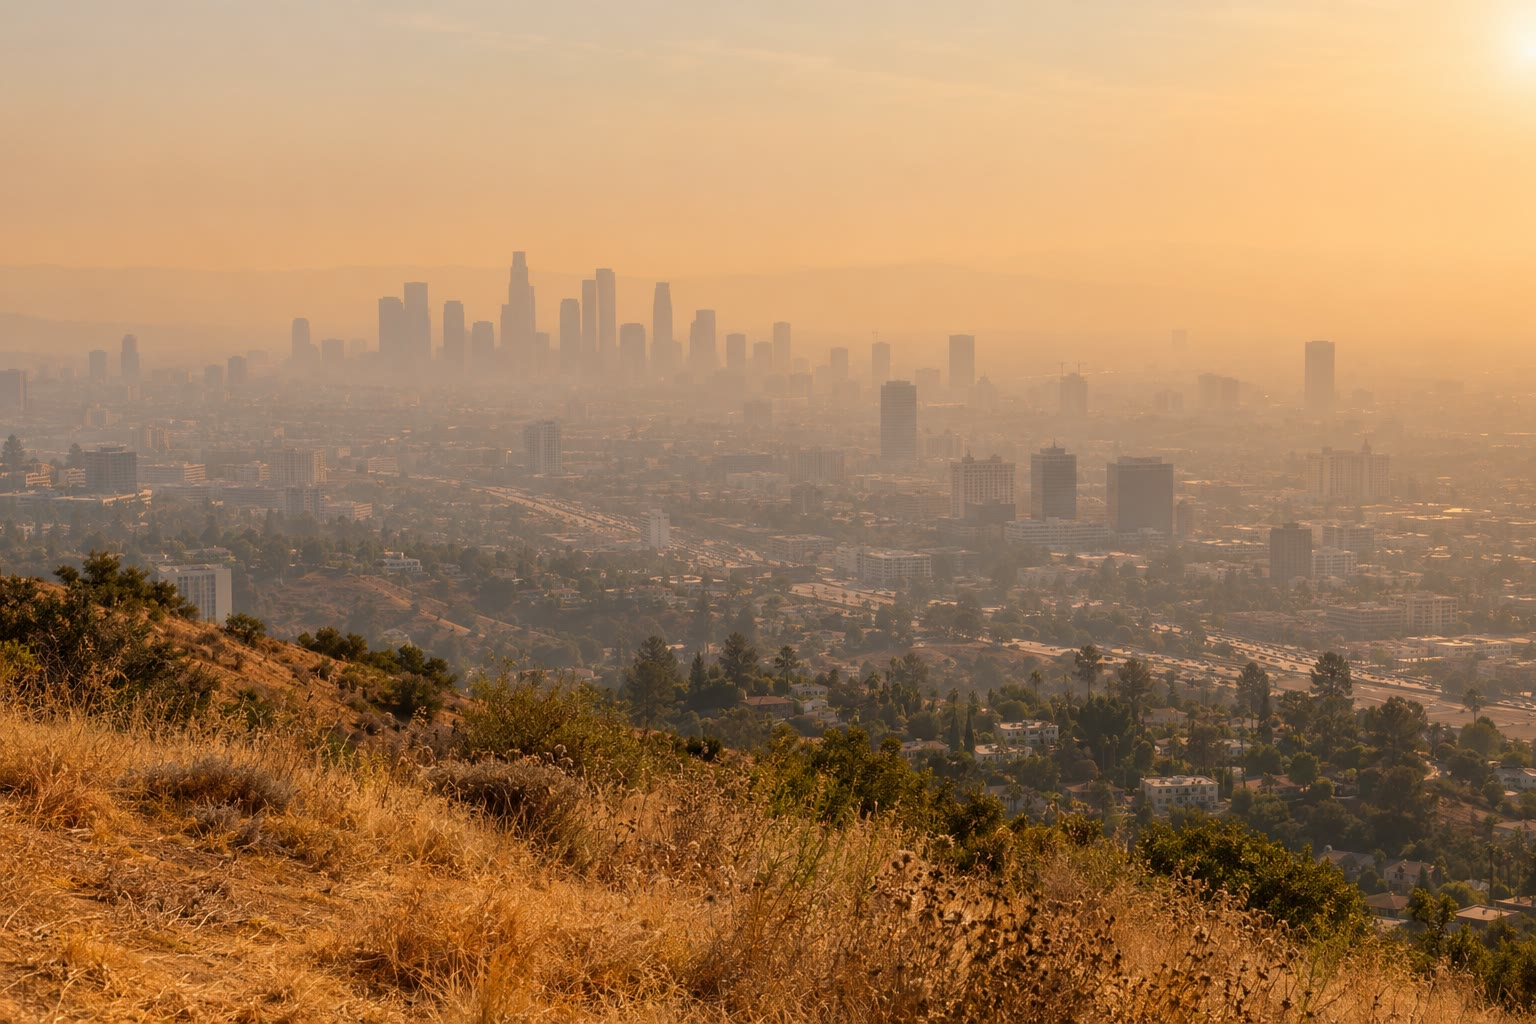
\includegraphics[width=0.6\linewidth]{images/book4/ai/b3-14-smog.jpg}

{\small Een stad onder \omterm{def:b3:photochemistry:smog}{fotochemische smog} op een hete namiddag. De bruine
tint komt van \ce{NO2}; de ozon, die de longen irriteert, is onzichtbaar.}
\end{omfigure}

\begin{omfigure}
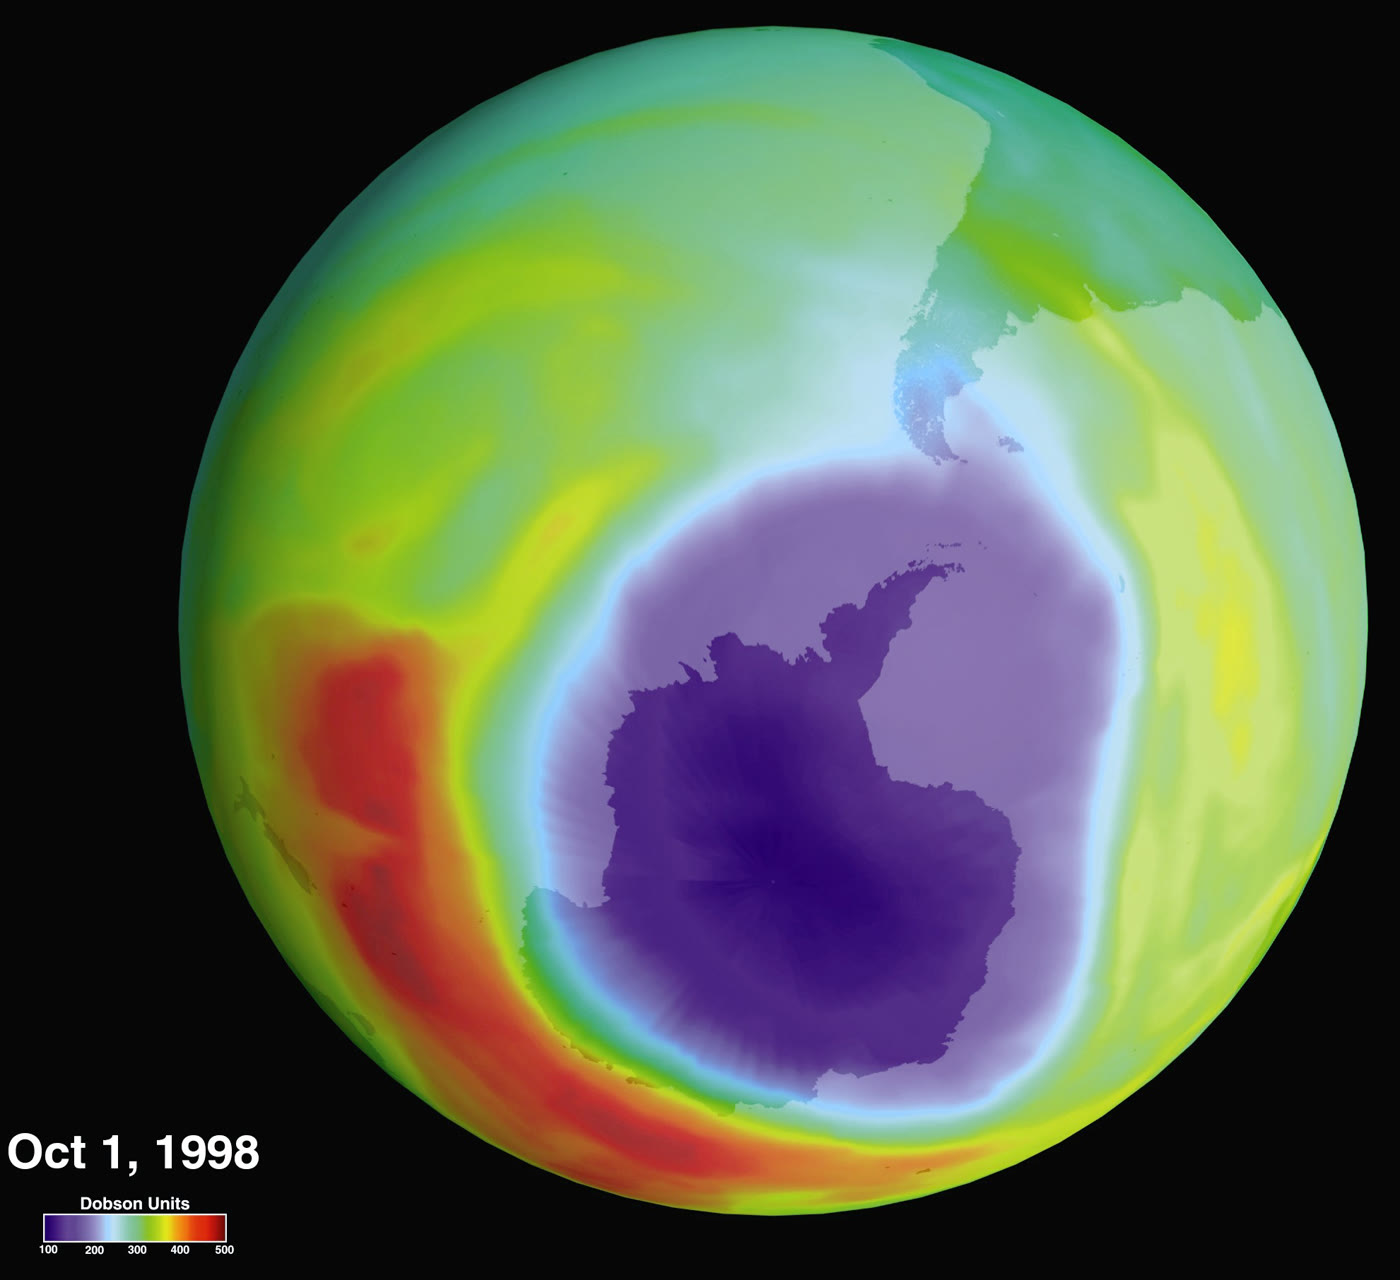
\includegraphics[width=0.5\linewidth]{images/book4/ozone-hole.jpg}

{\small De ozonkolom boven het zuidelijk halfrond op 1 oktober 1998, uit
satellietmetingen: het ozongat boven Antarctica (paars) zakt tot ongeveer
100 dobsoneenheden, tegenover ongeveer 300 elders.}
\end{omfigure}

\begin{inthelab}[Een fotoreactor]
Een middendrukkwiklamp, gekoeld in een kwartsmantel, staat in het midden
van het reactievat; een filterhuls van glas verwijdert de golflengten
onder ongeveer \qty{300}{nm}, die de producten zouden vernietigen. De
oplossing wordt met een stroom stikstof zuurstofvrij gemaakt (zuurstof
dooft tripletten uit) en geroerd. De hele reactor is afgeschermd: de lamp
zendt ultraviolet licht uit dat schadelijk is voor ogen en huid, en men
kijkt er nooit naar, zelfs niet even.
\end{inthelab}

\begin{safety}{\ghs[0.8cm]{GHS08}\ghs[0.8cm]{GHS09}}
% ledger: ghs4:benzophenone
Benzofenon, een gangbare sensibilisator en de beginstof van de
fotoreductie: verdacht van het veroorzaken van kanker, kan organen
beschadigen bij langdurige blootstelling, giftig voor in het water levende
organismen. Afwegen en hanteren met handschoenen; resten gaan naar het
organisch afval.
\end{safety}

\begin{history}[De fotochemie van de toekomst, en het gat in de hemel]
In 1912 vroeg Giacomo Ciamician zich in Bologna af of de industrie ooit,
zoals de planten, op zonlicht zou kunnen draaien in plaats van op steenkool;
hij had jarenlang kolven met organische verbindingen op het dak van zijn
laboratorium aan de zon blootgesteld. In 1985 meldden drie wetenschappers
die op een onderzoeksstation op Antarctica werkten, dat de ozonkolom
erboven in de lente sinds het einde van de jaren 1970 sterk afnam.
Het ozongat, binnen enkele jaren verklaard door de chemie van dit
hoofdstuk, leidde tot het uitfaseren van chloorfluorkoolwaterstoffen.
\end{history}

\section{Oefeningen}

\begin{exercise}[$\star$]\label{exo:b3:photochemistry:1}
Een lamp levert \qty{100}{mW} bij \qty{365}{nm}. Hoeveel fotonen per
seconde, en hoeveel einstein per seconde?
\end{exercise}

\begin{exercise}[$\star$]\label{exo:b3:photochemistry:2}
In \qty{10.0}{min} zet een oplossing die \qty{1.00e-7}{einstein.s^{-1}}
absorbeert
\qty{2.0e-5}{mol} beginstof om. Bereken de \omterm{def:b3:electronic-spectroscopy:quantum-yield}{kwantumopbrengst}.
\end{exercise}

\begin{exercise}[$\star$]\label{exo:b3:photochemistry:3}
De fotochemische reactie van \ce{H2} met \ce{Cl2} heeft \omterm{def:b3:electronic-spectroscopy:quantum-yield}{kwantumopbrengsten}
tot $10^4$ en meer. Wat toont dat aan? Schrijf de propagatiestappen op.
\end{exercise}

\begin{exercise}[$\star$]\label{exo:b3:photochemistry:4}
% ledger: janaf:O.dfH0, janaf:O3.dfH0
Bereken uit de vormingsenthalpieën bij 0 K van O (\qty{246.79}{kJ/mol}) en
\ce{O3} (\qty{145.35}{kJ/mol}) de grootste golflengten die \ce{O2} in twee
atomen kunnen splitsen en \ce{O3} in \ce{O2} en O.
\end{exercise}

\begin{exercise}[$\star\star$]\label{exo:b3:photochemistry:5}
Een fotoschakelaar heeft bij \qty{365}{nm} $\varepsilon_E = 22\,000$ en $\varepsilon_Z = 1500$ \unit{L.mol^{-1}.cm^{-1}}, met
$\Phi_{E\to Z} = 0.11$ en $\Phi_{Z\to E} = 0.40$ (gegevens van de oefening).
Bereken de fotostationaire samenstelling.
\end{exercise}

\begin{exercise}[$\star\star$]\label{exo:b3:photochemistry:6}
Geef de producten van de \omterm{def:b3:photochemistry:norrish}{norrishreactie van type II} van hexaan-2-on, en
leg uit waarom pentaan-2-on etheen geeft in plaats van propeen.
\end{exercise}

\begin{exercise}[$\star\star$]\label{exo:b3:photochemistry:7}
Een acceptor heeft een tripletenergie van \qty{250}{kJ/mol}. Welke van drie
kandidaat-sensibilisatoren met tripletenergieën van 289, 253 en
\qty{236}{kJ/mol} (gegevens van de oefening) draagt efficiënt over? Schat
voor elk de evenwichtsconstante van de overdracht bij \qty{298}{K}.
\end{exercise}

\begin{exercise}[$\star\star$]\label{exo:b3:photochemistry:8}
% ledger: kin:O+O2+M.k0, kin:O+O2+M.n
Bereken bij \qty{230}{K}, met $[\mathrm M] = \qty{4.0e17}{cm^{-3}}$, $[\ce{O2}] = 0.21[\mathrm M]$ en $j_3 = \qty{1.0e-3}{s^{-1}}$,
$k_2$ en de stationaire verhouding $[\ce{O}]/[\ce{O3}]$.
\end{exercise}

\begin{exercise}[$\star\star$]\label{exo:b3:photochemistry:9}
% ledger: kin:Cl+O3.A, kin:Cl+O3.EaR, kin:Cl+CH4.A, kin:Cl+CH4.EaR
Bereken bij \qty{230}{K} de snelheidsconstanten van $\ce{Cl + O3}$ en $\ce{Cl + CH4}$, en de
waarschijnlijkheid dat een Cl-atoom \ce{O3} ontmoet in plaats van \ce{CH4}
wanneer $[\ce{O3}] = \qty{5.7e12}{cm^{-3}}$
en $[\ce{CH4}] = \qty{4.0e11}{cm^{-3}}$.
\end{exercise}

\begin{exercise}[$\star\star\star$]\label{exo:b3:photochemistry:10}
% ledger: kin:NO+O3.A, kin:NO+O3.EaR
Rond het middaguur is in een stad $[\ce{NO2}]/[\ce{NO}] = 1.5$ en $j_{\ce{NO2}} = \qty{8.0e-3}{s^{-1}}$. Bereken de
fotostationaire ozon bij \qty{298}{K} in moleculen per \unit{cm^3} en in
ppb (lucht bij \qty{1}{bar}). Wat gebeurt er 's nachts?
\end{exercise}

\begin{exercise}[$\star\star\star$]\label{exo:b3:photochemistry:11}
Een oplossing van \qty{3.0}{mL} met absorbantie 0.50 bij \qty{313}{nm}
ontvangt \qty{50}{mW} licht met die golflengte; de reactie heeft $\Phi = 0.25$. Bereken de beginsnelheid in
\unit{mol.L^{-1}.s^{-1}}.
\end{exercise}

\begin{exercise}[$\star\star\star$]\label{exo:b3:photochemistry:12}
Een ferrioxalaatactinometer, met een \omterm{def:b3:electronic-spectroscopy:quantum-yield}{kwantumopbrengst} van 1.25 bij
\qty{365}{nm} (gegevens van de oefening) en volledige absorptie, vormt
\qty{3.0e-6}{mol} Fe(II) in \qty{60}{s}. Bereken de \omterm{def:b3:photochemistry:photon-flux}{fotonenflux}. Waarom
moet de omzetting klein blijven?
\end{exercise}

\section{Probleem: de ozonlaag maken en afbreken}

\begin{problem}[{Weekendprobleem --- de ozonlaag maken en afbreken:
fotondrempels, de stationaire toestand van Chapman met geëvalueerde
snelheidsconstanten, de chloorcyclus, en de reservoirs die hem stoppen}]
\label{pb:b3:photochemistry:1}
% ledger: janaf:O.dfH0, janaf:O3.dfH0, kin:O+O2+M.k0, kin:O+O2+M.n, kin:O+O3.A, kin:O+O3.EaR, kin:Cl+O3.A, kin:Cl+O3.EaR, kin:O+ClO.A, kin:O+ClO.EaR, kin:Cl+CH4.A, kin:Cl+CH4.EaR, kin:ClO+NO2+M.k0, kin:ClO+NO2+M.n, kin:ClO+NO2+M.kinf, kin:ClO+NO2+M.Fc, oz:column.mean, oz:column.hole
Een model van de stratosfeer rond \qty{30}{km} (gegevens van het probleem): $T = \qty{230}{K}$, $[\mathrm M] =
\qty{4.0e17}{cm^{-3}}$, $[\ce{O2}] = 0.21[\mathrm M]$, \omterm{def:b3:photochemistry:photolysis}{fotolysesnelheidsconstanten} $j_1 = \qty{1.0e-11}{s^{-1}}$ (\ce{O2})
en $j_3 = \qty{1.0e-3}{s^{-1}}$ (\ce{O3}), $[\ce{CH4}] = \qty{4.0e11}{cm^{-3}}$, $[\ce{NO2}] = \qty{1.0e9}{cm^{-3}}$. Geëvalueerde
snelheidsconstanten (\unit{cm^3.s^{-1}}, of \unit{cm^6.s^{-1}} voor $k_2$,
met concentraties geteld per \unit{cm^3}):
$k_2 = \num{6.0e-34}(T/300)^{-2.6}$; $k_4 = \num{8.0e-12}\eu^{-2060/T}$; Cl + \ce{O3}: $\num{2.8e-11}\eu^{-250/T}$;
O + ClO: $\num{2.5e-11}\eu^{110/T}$; Cl + \ce{CH4}: $\num{6.6e-12}\eu^{-1240/T}$; ClO + \ce{NO2} + M: $\num{1.41e-13}$ onder
deze omstandigheden.

\medskip\noindent\textbf{Deel I --- Fotondrempels.}
\begin{enumerate}
  \item Bereken $D_0(\ce{O2})$ uit $\Delta_fH^\circ_0(\ce{O}) = \qty{246.79}{kJ/mol}$.
  \item Leid de grootste golflengte af die \ce{O2} splitst.
  \item Bereken de energie van $\ce{O3 -> O2 + O}$ ($\Delta_fH^\circ_0(\ce{O3}) = \qty{145.35}{kJ/mol}$) en
        haar drempelgolflengte.
  \item Zichtbaar licht zou ozon dus kunnen splitsen; waarom is het de
        ultraviolette absorptie van ozon die telt voor het leven?
  \item Waarom wordt \ce{O2} alleen hoog in de atmosfeer gefotolyseerd?
\end{enumerate}

\medskip\noindent\textbf{Deel II --- De stationaire toestand van Chapman.}
\begin{enumerate}[resume]
  \item Schrijf de vier stappen van Chapman op.
  \item Bereken $k_2$ en $k_2[\mathrm M]$ bij \qty{230}{K}.
  \item Bereken $k_4$.
  \item Bereken $[\ce{O}]/[\ce{O3}]$.
  \item Toon aan dat $[\ce{O3}] = [\ce{O2}]\sqrt{j_1k_2[\mathrm M]/(j_3k_4)}$.
  \item Bereken $[\ce{O3}]$ en zijn mengverhouding.
  \item Bereken $[\ce{O}]$.
  \item De waargenomen ozon is lager dan dit. Waarom?
\end{enumerate}

\medskip\noindent\textbf{Deel III --- De chloorcyclus.}
\begin{enumerate}[resume]
  \item Schrijf de cyclus en zijn nettoreactie op.
  \item Bereken de levensduur van een Cl-atoom ten opzichte van \ce{O3}.
  \item Bereken de levensduur van ClO ten opzichte van O.
  \item Leid de stationaire verhouding $[\ce{ClO}]/[\ce{Cl}]$ af.
  \item Vergelijk, met $[\ce{Cl}] + [\ce{ClO}] = \qty{1.0e7}{cm^{-3}}$, de
        snelheid van het verlies aan oneven zuurstof door de cyclus met die
        van de stap van Chapman $\ce{O + O3}$.
  \item Welke stap beperkt de cyclus?
\end{enumerate}

\medskip\noindent\textbf{Deel IV --- De reservoirs.}
\begin{enumerate}[resume]
  \item Bereken de waarschijnlijkheid dat een Cl-atoom met \ce{O3} reageert
        in plaats van met
        \ce{CH4}.
  \item Bereken de waarschijnlijkheid dat ClO met O reageert in plaats van
        met \ce{NO2}.
  \item Leid de waarschijnlijkheid $p$ af dat een omloop van de cyclus
        voltooid wordt.
  \item Leid het gemiddelde aantal omlopen af voordat het chloor gevangen
        wordt.
  \item Leg uit hoe polaire stratosferische wolken de keten verlengen.
  \item Formuleer het resultaat: het aantal ozonmoleculen dat één
        chlooratoom in dit model vernietigt voordat het in een reservoir
        gevangen wordt.
\end{enumerate}
\end{problem}
